\section{Method}

This thesis uses the \acf{DSRM}. \Ac{DSRM} itself is based on the \textit{Design science} paradigm, described by \citeauthor{Simon1988} \autocite{Simon1988}. \citeauthor{Hevner2004} \autocite{Hevner2004} explain that design science involves the creation and evaluation of information technology artifacts aimed at addressing specific organizational issues. These artifacts can take various forms, ranging from software, formal logic, mathematical models, to informal language descriptions. The mathematical foundation of the design process enables various forms of quantitative evaluations of IT artifacts, including optimization, analytical simulations, and comparative assessments with alternative design options.

Based on the \ac{DSRM} process illustrated by \citeauthor{Peffers2007} in \cref{fig:dsrm_process}, the research entry point for this thesis will be the \textit{Design \& Development Centered Initiation}. The problem, as well as the motivation, are both already well-defined and are outlined in \cref{subsection:problem}: the \ac{DoHG@MHH} needs to switch the genetic analysis pipeline to a newer reference genome, presenting multiple challenges to overcome. The \textit{objectives of a solution} (see \cref{fig:dsrm_process}) are outlined in \cref{subsection:goals}: professionalization of pipeline utilization and potential usage of cloud services. Both should be accomplished by introducing a \ac{SWfMS} to the genetic analysis pipeline. There is no quantitative goal to reach~\textemdash~all improvements are considered valuable. Nevertheless, the outcome should outweigh the investment, therefore pipeline runtime and resource usage will be evaluated. Although accessibility and usability are needed, given that the pipeline will be used by biologists and medical staff, those soft features will not be assessed.

This makes the following steps the research focus of this thesis:
\begin{description}
    \item[Design \& Development] \Cref{sec:artifact_description} will document the transition from shell scripts to a \ac{SWfMS}. The choice of \ac{SWfMS} (\textit{design search process}, see \autocite{Gregor2013}) based on the \nameref{sec:literature_review} (\cref{sec:literature_review}) will be outlined as well.
    \item[Demonstration] The translated pipeline will be run, and the results will be compared to already existing reference results to validate the correct usage as part of the \textit{Design \& Development} process.
    \item[Evaluation] Runtime and resource usage of the pipeline run by the \ac{SWfMS} will be measured and compared to previous versions of the pipeline as part of the \lowercase{\nameref{sec:artifact_description}} in \cref{sec:artifact_description}. The results will also be discussed in \cref{sec:discussion}.
\end{description}
As the evaluation of the resource usage of the \ac{SWfMS} will give some meaningful insights for optimization, \cref{sec:artifact_description} will iterate upon these steps to reach a satisfactory outcome.

Additionally, the structure of this thesis closely follows the publication schema for a \ac{DSR} study, described by \citeauthor{Gregor2013} \autocite[Table 3]{Gregor2013}. Following their example, the closing sections, \nameref{sec:discussion} (\cref{sec:discussion}) and \nameref{sec:conclusion} (\cref{sec:conclusion}), will be used to bolster the research rigorousness of this thesis.

\begin{figure}[H]
    \centering
	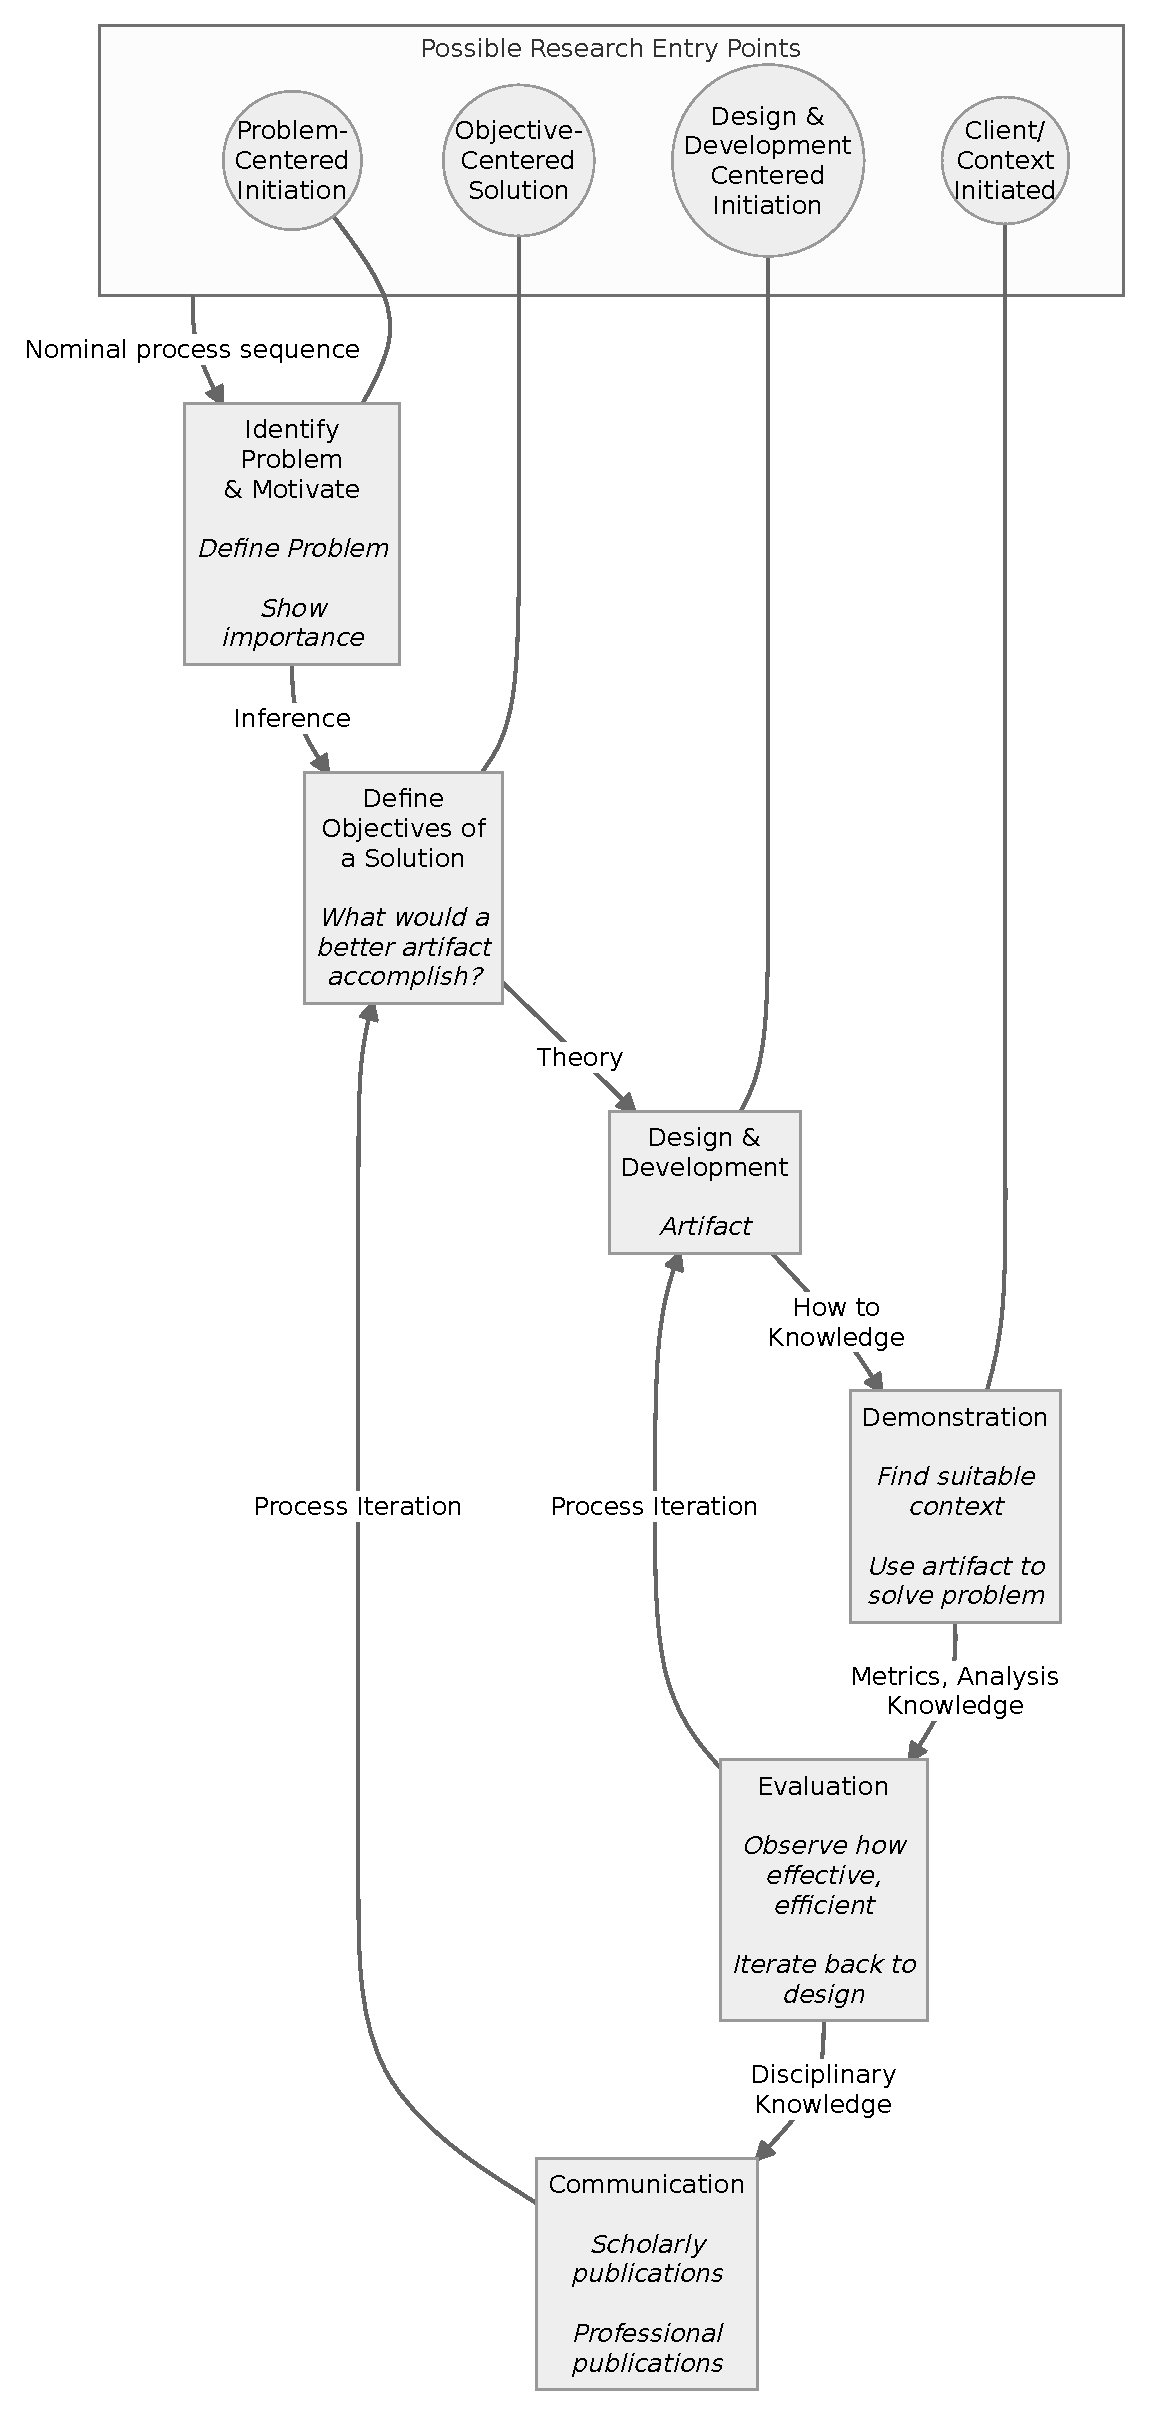
\includegraphics[width=0.9\textwidth,height=0.9\textheight,keepaspectratio]{flowcharts/dsrm_process.pdf}
	\caption[\ac{DSRM} Process Model]{\ac{DSRM} process model}{Based on \autocite[Figure 1]{Peffers2007}.}
	\label{fig:dsrm_process}
\end{figure}
